\section{KC3DDIODE: The Diode Toolbox}
The module \textbf{kc3ddiode} contains parametric models
of diodes. The models are as follows:

\begin{itemize}
\item \textbf{do35}: DO-35 package glass encapsulated axial diode
\item \textbf{GenDiode}: Generic tubular axial diode
\end{itemize}

\begin{figure}
\label{fig:k3ddiode-diodes}
\centering
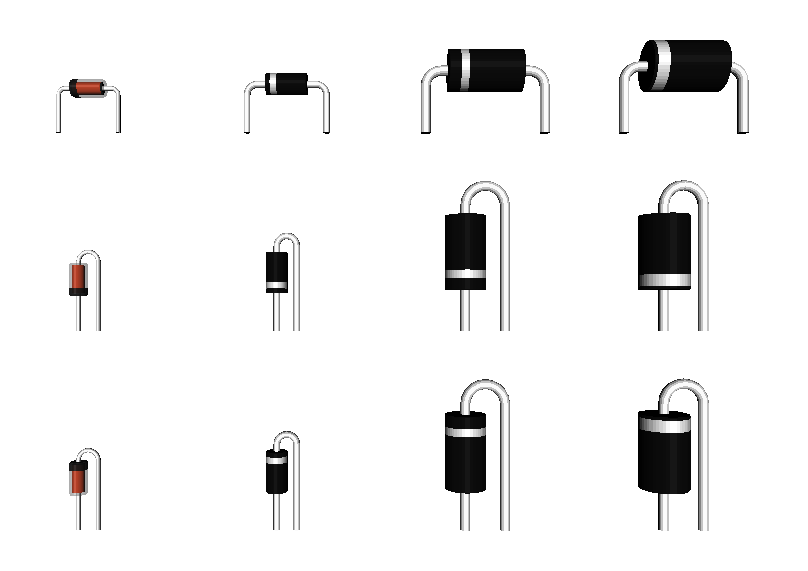
\includegraphics[width = 0.8\textwidth]{img/k3ddiode.png}
\caption{Glass encapsulated diodes (do35) produced via the do35 model;
DO-41, DO-201, and DO-204 models produced via the GenDiode model.}
\end{figure}

\subsection{kc3ddiode:do35}
The class \textbf{do35} represents a DO-35 package glass encapsulated
axial diode such as the 1N4148. Most parameters are fixed according
to the DO-35 specification but the user has some control of the
material appearance, lead pitch, and orientation. The dimensions used
are the Maximum Material Condition specifications. The public methods
include:

\textbf{setColors(wirecolor, glasscolor, cathodecolor, tubecolor)}
where the arguments are the filenames for material appearance specifications
(VRMLMat files). The wirecolor controls the appearance of the lead,
glasscolor controls the appearance of the glass envelope,
cathodecolor controls the appearance of the cathode band, and
tubecolor controls the appearance of the metallic tube inside the
glass envelope.

\textbf{setNVertices(wire, tube, bend)} where wire is the number of
vertices to use for the wire's cross-section, tube is the number of
vertices to use in the cross-section of the envelope and tube,
and bend is the number of segments in a bend.

\textbf{build(partname, scale, horiz, vflip, pitch, lead)}: create the
3D model; partname is the name of the part and also the base name of the
output file; it must contain only the characters a..z, A..Z, 0..9, and the 
underscore character and the first character must be an alphabetic character.
scale is the scale factor; since the internal units are in mm, use a scale of
0.3937 to produce a model for use in the KiCAD 3D viewer. horiz must be set to
True for horizontal orientation; when the orientation is vertical, vflip may
be set to True to place the cathode at pin 2. pitch is the lead pitch and
lead is how far the lead protrudes below the top of the PCB.

The example below creates a DO-35 package diode in a horizontal orientation,
in which the cathode is always pin 1, and in two vertical orientations in which
the cathode is first on pin 1 and then on pin 2.

\begin{verbatim}
import kc3d
from kc3d import *
import kc3ddiode
from kc3ddiode import *

diode = do35()
diode.setNVertices(16, 48, 5)
diode.setColors("../colors/tin.mat", "../colors/glass_clr.mat",
    "../colors/glass_blk.mat", "../colors/copper.mat")

# horizontal with 0.3" pitch; the cathode is always pin 1
diode.build("do35_0I300H", 0.3937, True, False, 7.62)

# we must double the number of bend segments in the
# vertical orientation since we have a 180 degree bend
# rather than 90 degree bends:
diode.setNVertices(16, 48, 10)

# vertical with 0.1" pitch, the cathode is pin 1
diode.build("do35_0I100V", 0.3937, False, False, 2.54)

# vertical with 0.1" pitch, the cathode is pin 2
diode.build("do35_0I100VK2", 0.3937, False, True, 2.54)
\end{verbatim}


\subsection{kc3ddiode:GenDiode}
The class \textbf{GenDiode} represents a generic tubular axial diode;
the model has been used to generate 3D models of diodes with the
DO-41, DO-201, and DO-204 package specifications. Since the dimensions
are not hard-coded as in the case of the do35 model, the output is
not strictly limited to the Maximum Material Condition of any particular
package specification. The public methods
include:

\textbf{setColors(wirecolor, bodycolor, cathodecolor)}
where the arguments are the filenames for material appearance specifications
(VRMLMat files). The wirecolor controls the appearance of the lead,
bodycolor controls the appearance of the envelope, and
cathodecolor controls the appearance of the cathode band.

\textbf{setNVertices(wire, tube, bend)} where wire is the number of
vertices to use for the wire's cross-section, tube is the number of
vertices to use in the cross-section of the envelope and tube,
and bend is the number of segments in a bend.

\textbf{build(partname, scale, horiz, vflip, pitch, lead)}: create the
3D model; partname is the name of the part and also the base name of the
output file; it must contain only the characters a..z, A..Z, 0..9, and the 
underscore character and the first character must be an alphabetic character.
scale is the scale factor; since the internal units are in mm, use a scale of
0.3937 to produce a model for use in the KiCAD 3D viewer. horiz must be set to
True for horizontal orientation; when the orientation is vertical, vflip may
be set to True to place the cathode at pin 2. pitch is the lead pitch and
lead is how far the lead protrudes below the top of the PCB.

\textbf{setParams(wire, body, length, band, space)}: set the dimensions of the
package; wire is the wire diameter, body is the tube (body) diameter, length
is the tube's length, band is the width of the cathode band, and space is the
distance between the edge of the tube and the diode band.

The example below creates a DO-41 package diode in Maximum Material Condition
in a horizontal orientation and two vertical orientations:

\begin{verbatim}
# load the tools
import kc3d
import kc3ddiode
from kc3d import *
from kc3ddiode import *

diode = GenDiode()
diode.setNVertices(16, 48, 5)
#DO41 has max material for dwire = 0.864, dbody = 2.72, lbody = 5.21
diode.setParams(0.864, 2.72, 5.21, 0.8, 0.6)
diode.setColors("../colors/tin.mat", "../colors/rcc_blk_g.mat", "../colors/rcc_wht_g.mat")

# horizontal orientation (pin 1 is always the cathode)
diode.build("do41_0I400H", 0.3937, True, False, 10.16)

diode.setNVertices(16, 48, 10)

# vertical orientation, pin 1 is the cathode
diode.build("do41_0I100V", 0.3937, False, False, 2.54)

# vertical orientation, pin 2 is the cathode
diode.build("do41_0I100VK2", 0.3937, False, True, 2.54)
\end{verbatim}
